\documentclass{article}
\usepackage{amsmath,amsfonts,amsthm,amssymb}
\usepackage{enumerate}
\usepackage[shortlabels]{enumitem}
\usepackage{algorithm}
\usepackage{algpseudocode}
\usepackage{bbm}
\usepackage{float}
\usepackage{framed}
\usepackage{mathrsfs}
\usepackage{cite}
\usepackage{url}
\usepackage{multirow}
\usepackage{siunitx}
\usepackage{hyperref}
\usepackage{graphicx}

\def\zt{\mathbb{Z}/t\mathbb{Z}}
\def\*#1{\mathbf{#1}}

\newtheorem{thm}{Theorem}
\newtheorem{lem}{Lemma}
\newtheorem{prb}{Problem}

\title{%
  Algorithms for Evaluating Nonlinear Functions Under Homomorphic Encryption
}
\author{Trevor Henderson\\{\small Applied Cryptography Group}\\{\small Orange Labs, Caen, France}}
\date{August 30, 2016}

\begin{document}

\maketitle

    \begin{abstract}

        This paper investigates methods of computing nonlinear functions efficiently
        under the constraints of common fully homomorphic encryption schemes
        --- access to only addition and multiplication modulo $t$.
        I show that $\sqrt{t}$ multiplications are necessary 
        and $3\sqrt{t}$ multiplications are sufficient to evaluate
        a general single variable function.
        I then show that many multivariate functions, such as division
        and boolean comparisons can also be evaluated using
        $O(\sqrt{t})$ multiplications.
        The multiplicative depth of both algorithms is $O(\log t)$.
        Despite meeting asymptotic lower bounds,
        it is disappointing to learn that
        any reasonably complex homomorphic function is necessarily weakly polynomial.
        This suggests that more flexible encryption schemes must be pursued if
        homomorphic encryption is to become practical.

        Experimental results utilizing an 
        implementation of the somewhat homomorphic scheme,
        YASHE, demonstrate
        secure, homomorphic evaluations of arbitrary
        8-bit single variable functions 
        in less than 4 milliseconds amortized
        on a 2012 MacBook Pro.
        Test scenarios that could be useful in cloud computing,
        such as converting an image from RGB
        to YCbCr color formats and applying color filters,
        are computed in minutes.
        Both of these results show significant improvement over the
        state of the art.
    \end{abstract}

    \section{Introduction}
        Put simply, homomorphic encryption allows one to encrypt messages
        and then
        perform math on these encrypted messages without revealing the contents~\cite{firstImp}.
        Researchers speculate that if the field becomes practically feasible it could revolutionize the security of cloud computing~\cite{cloud}.
        For example, imagine a search engine that allowed you to encrypt a query with homomorphic encryption before sending it to the server.
        The server would perform some sort of computation on your query to transform it into a list of results,
        and then send the results back to you without ever knowing what it was that you searched for!


        Many commonly used encryption schemes, like RSA, are \emph{partially homomorphic} because they
        allow for some, but not all, operations to be performed on the encrypted texts~\cite{rivest}.
        However, for many decades it remained an unsolved problem as to whether there exists
        a \emph{fully homomorphic} encryption scheme --- a scheme where any operation can be performed
        on the encrypted texts~\cite{rivest}.
        In 2013, Craig Gentry's groundbreaking work~\cite{homenc,firstImp} demonstrated that this ``holy grail'' of cryptography~\cite{grail}
        does, in fact, exist.

        This discovery and most derivative schemes~\cite{homenc,firstImp,yashe,faster,shorter,lwe,depth,leveled,gapsvp,smaller,integers},
        obey the following format.
        The plaintext is encrypted with some sort of noise.
        As homomorphic operations are performed this noise grows until,
        after a certain amount of computation,
        it becomes so large that the ciphertext can no longer be decrypted.
        To mitigate this,
        a procedure called \emph{bootstrapping} decrypts and re-encrypts the text,
        entirely with homomorphic operations, resetting the noise to some small constant.
        By continuing to apply bootstrapping whenever necessary, an arbitrary number
        of operations can be performed.
        However, this comes with an immense computational overhead.
        So, in practice, many schemes are \emph{somewhat homomorphic}~\cite{firstImp,homenc}.
        These schemes do not bootstrap, which bounds the number of operations that can be performed
        before the text deteriorates.

        In early work,
        homomorphic encryption was reported to be extremely slow, with
        single bit operations taking as long as half an hour to compute~\cite{firstImp}.
        Recent advancements allow large circuits to be evaluated in seconds~\cite{yashe,somewhat}.
        But still, these circuits are limited to consist of only addition and multiplication operations.
        Although any function can theoretically be computed with these operations~\cite{homenc},
        it is not obvious how to do so efficiently~\cite{newton,aes,genomic,fixedpoint}.

        This paper investigates ways of computing these nonlinear
        functions including
        boolean comparisons and division under a particular model of homomorphic computing.
        In section~\ref{desc}, the specific constraints of this model are established.
        Section~\ref{high} provides a solution to this proposed problem and proves the solution is asymptotically optimal.
        Section~\ref{multi} expands these results to include multivariate functions.
        Finally, section~\ref{exp} provides experimental results and section~\ref{conc}
        concludes with a discussion of some of the inherent limitations of homomorphic encryption revealed by these results.

    \section{A Model of Homomorphic Computing}
    \label{desc}

    The goal of this work
    is to describe methods of evaluating functions over the integers modulo $t$ efficiently under homomorphic encryption.
    Setting aside the specifics of homomorphic schemes, 
    the constraints of many of them can be generalized as follows~\cite{homenc,yashe,somewhat,firstImp,smaller,integers,faster,shorter,lwe,depth,leveled,gapsvp}:
    \begin{enumerate}[1.]
        \item
            The available operations are addition and multiplication modulo the plaintext modulus, $t$.
        \item
            Additions and scalar multiplications are relatively easy to compute, where as nonscalar multiplications are much harder to compute. 
        \item
            Additions and scalar multiplications do not increase the noise of ciphertexts by much, whereas nonscalar multiplications greatly increase the noise of ciphertexts.
    \end{enumerate}

    Therefore, in order to evaluate functions efficiently, the computation must minimize
    the total number of nonscalar multiplications (reducing the total computation time),
    as well as the nonscalar multiplicative depth (reducing the overhead associated with noise growth).

    \subsection{Limitations of this model}
        Naturally, this model does not cover all cases as there are many homomorphic schemes,
        some of which have additional properties that can ease computation.
        For example, some configurations allow the individual bits of ciphertexts to be
        accessed and computed upon~\cite{aes,newton,genomic}.
        This make
        it possible to implement standard computer hardware algorithms that rely on bit shifting and bit logic to perform operations like evaluating inequalities and performing division.

        Additionally, there are homomorphic schemes that support plaintext moduli so large that performing integer multiplications to the maximum multiplicative depth will not cause overflow.
        Under these schemes one can perform floating point operations by keeping track of a radix index for each integer and scaling down the decrypted result appropriately~\cite{newton,fixedpoint}.
        
        While these alternatives are freeing, they currently come at enormous cost.
        In the bit method, the ciphertexts only encrypt single integers,
        making them orders of magnitude less efficient than schemes that use batch processing.
        As for ciphertexts that do not overflow, they must be immense in size, again sacrificing valuable performance.
        %Still, these methods are useful in areas where complicated homomorphic functions must be calculated on only a few, large inputs but I will not discuss them further.
        %Additionally, from a purely aesthetic standpoint, adding other helper variables 
        %like a radix, 
        %takes away from some of the magic of homomorphic computation. 
        %It is far less amazing to unbox something half finished,
        %than it is to have a solution appear all at once and ready to go.


    \section{Evaluating Single-Variable Functions}
    \label{high}

        The key insight of my proposed solution is to form
        a more symbiotic relationship with the modulo operation that is built
        into the homomorphic addition and multiplication operations.
        I show that this modulus can be used as a tool for simplification, rather than a boundary that must be avoided, as in~\cite{newton, fixedpoint}.

        Using this philosophy I will derive a method to compute any single variable homomorphic function. 
        In section~\ref{notation}, I establish notation,
        in section~\ref{comp} I discuss the conditions under which single variable functions are computable,
        and in~\ref{bounds} I discuss the algorithms that compute them and their complexity.

        %This method can efficiently perform batch operations on relatively small 
        %(8 or 16-bit) integers. 
        %This makes it very useful for problems like image processing.

    \subsection{Notation}
    \label{notation}
        For clarity, the proofs and discussion to below use the following notation:
        \begin{enumerate}[-]
            \item
                A function is \emph{computable} if it can be computed using only addition and multiplication operations modulo $t$.
            \item
                All homomorphically encrypted variables are represented in \textbf{bold}.
            \item
                All operations are assumed to be modulo $t$ and equality ``$=$'' is used to represent congruence modulo $t$.
            \item
                $\delta: \zt\to\{0,1\}$ is the standard Dirac delta function, modulo $t$:
                \begin{align}
                    \delta(x) =
                    \left\{
                        \begin{array}{cc}
                            1 & \text{if } x = 0\\
                            0 & \text{if } x \neq 0
                        \end{array}
                    \right.
                \end{align}
        \end{enumerate}

    \subsection{Computability of Single-Variable Functions}
    \label{comp}
    In lemmas~\ref{lem1} and~\ref{lem2}, I establish, through construction, that it is possible to compute any function with the given operations if the modulus, $t$, is prime.
    Lemmas~\ref{lem3} and~\ref{lem4} go on to enumerate the number distinct functions that exist as well as the number of ways that these functions can be computed.
    Theorem~\ref{thm1} concludes through a counting argument that all functions are computable if and only if the modulus $t$ is prime,
    and furthermore that each of these functions has a unique polynomial that computes it.

    \begin{lem}
      \label{lem1}
        If $\delta$ is computable, then any total function 
        $f:\zt\to\zt$ is computable.
    \end{lem}
    \begin{proof}
        Using the function $\delta$, any total function $f:\zt\to\zt$ can be computed as follows:
        \begin{align}
            f(x) = \sum_{k = 0}^{t-1} f(k)\delta(x - k)
        \end{align}
    \end{proof}
    
    \begin{lem}
      \label{lem2}
        $\delta$ is computable if $t$ is prime.
    \end{lem}
    \begin{proof}
        If $t$ is prime then $\delta$ can be computed as follows:
        \begin{align}
            \delta(x) = 1 - x^{t - 1}
        \end{align}
        By Fermat's Little Theorem~\cite{numbers}, if $x \neq 0$ then $x^{t - 1} = 1$ and so $\delta(x) = 0$.
        If $x = 0$, then $x^{t - 1} = 0$ and so $\delta(x) = 1$. 
    \end{proof}

    \begin{lem}
      \label{lem3}
        Exactly $t^{t}$ distinct total functions $f:\zt\to\zt$ exist. 
    \end{lem}
    \begin{proof}
        Each of the $|\zt|$ possible inputs to $f$ corresponds to 
        one of $|\zt|$ possible outputs, therefore there are
        \begin{align}
            |\zt|^{|\zt|} = t^t
        \end{align}
        distict functions that exist. 
    \end{proof}

    \begin{lem}
      \label{lem4}
        At most $t^{\varphi(t) + 1}$ distinct total functions $f:\zt\to\zt$ are computable.
    \end{lem}
    \begin{proof}
      By Euler's Theorem~\cite{numbers}, $x^{\varphi(t) + 1} = x$, 
        therefore any polynomial $P$ can be reduced to the form
        \begin{align}
          P(x) = \sum_{i = 0}^{\varphi(t)} a_{i}x^{i}
        \end{align}
        This reduced polynomial has $\varphi(t) + 1$ coefficients, 
        each of which can take on one of $|\zt| = t$ values,
        therefore $t^{\varphi(t) + 1}$ such polynomials exist. 
        Any computation involving only addition and multiplication modulo $t$
        is equivalent to a polynomial modulo $t$, therefore at most
        $t^{\varphi(t) + 1}$ total functions can be computed. 
    \end{proof}

    \begin{thm}
      \label{thm1}
        All possible functions 
        $f:\zt\to\zt$ 
        can be computed if and only if $t$ is prime.
        Furthermore,
        if $t$ is prime, then each function 
        $f:\zt\to\zt$ 
        is uniquely represented by a polynomial of degree less than $t$. 
    \end{thm}
    \begin{proof}
      If $t$ is prime then $\delta$ can be computed by lemma~\ref{lem2}. So, by lemma~\ref{lem1}, all functions can be computed.
        If $t$ is not prime then $\varphi(t) + 1 < t$. So, by lemmas~\ref{lem3} and~\ref{lem4}
        there must exist some function that cannot be computed.

        If $t$ is prime, there are $t^{\varphi(t) +1} = t^t$ functions computable by polynomials and $t^t$ distinct functions.
        Since no two distinct functions can be computed in the same way each function must be uniquely represented by exactly one polynomial.
    \end{proof}

    \subsection{Complexity of Single-Variable Functions}
    \label{bounds}

    Given the analysis in the previous section,
    consider the modulus $t$ to be prime from this point forward.
    From the construction in lemma~\ref{lem1} and the definition of $\delta$ from lemma~\ref{lem2},
    we can calculate the minimal polynomial representing a function as follows:
    \begin{align}
        P(x) = \sum_{k = 0}^{t-1} f(k)\delta(x - k)\pmod{x^t - x}
    \end{align}
    Computing this polynomial takes $O(t^2F)$ time where $F$ is the complexity of $f(x)$.
    However, this computation occurs without any homomorphic overhead, so it can be considered negligible, for reasonable choices of $f$ and $t$.

    Theorem~\ref{thm1} proved that each function $f$ has a unique polynomial that computes it.
    Therefore, there is no faster way to calculate $f(x)$ than by evaluating $P$ at $x$.
    Paterson and Stockmeyer~\cite{paterson} proved that evaluating an arbitrary polynomial of degree
    $t$ requires at least $\sqrt{t}$ nonscalar multiplications.

    Algorithm~\ref{evalSinglePoly} is a modification of Paterson and Stockmeyer's Algorithm B that maintains a logarithmic multiplicative depth.
    It requires approximately $3\sqrt{t}$ nonscalar multiplications and has a multiplicative depth of $O(\log t)$.

    \begin{algorithm}
        \caption{Evaluate a single variable polynomial}\label{evalSinglePoly}
        \begin{algorithmic}
            \Function{EvaluatePolynomial}{$\mathbf{x}$, $P$}
                \\
                \State{
                  Let $P$ be a polynomial $a_0 + a_1x + \cdots + 
                  a_{t}x^{t}$ with 
                  $t = m^{2} - 1$
                }
                \\
                \State{
                  $\mathbf{X}[0] \leftarrow 1$, $\mathbf{X}[1] \leftarrow \mathbf{x}$
                }
                \Comment{$\mathbf{X}[i] = \mathbf{x}^i$}
                \\
                \For{$i = 2$ to $m$}
                    \State{
                      $\mathbf{X}[i] = 
                      \mathbf{X}\left[\left\lfloor\frac{i}{2}\right\rfloor\right]
                      \cdot
                      \mathbf{X}\left[\left\lceil\frac{i}{2}\right\rceil\right]$
                    }
                    \Comment{
                      Compute powers $\mathbf{x}^2 \dots \mathbf{x}^{m}$
                    }
                \EndFor%
                \\
                \For{$i = 2$ to $m-1$}
                    \State{
                      $\mathbf{X}[im] = 
                      \mathbf{X}\left[\left\lfloor\frac{i}{2}\right\rfloor m\right]
                      \cdot
                      \mathbf{X}\left[\left\lceil\frac{i}{2}\right\rceil m\right]$
                    }
                    \Comment{
                      Compute powers $\mathbf{x}^{2m}\dots \mathbf{x}^{(m-1)m}$
                    }
                \EndFor%
                \\
                \State{$\mathbf{p} \leftarrow 0$}
                \Comment{Compute the polynomial as}
                \For{$i = 0$ to $m-1$}
                \Comment{
                  $\sum_{i = 0}^{m-1}\mathbf{x}^{im}\left(\sum_{j = 0}^{m - 1}a_{im + j}\mathbf{x}^j\right)$
                }
                \State{$\mathbf{q} \leftarrow 0$}
                %\Comment
                %$(a_0 + a_1x + \dots a_{m-1}x^{m-1})$
                    \For{$j = 0$ to $m - 1$}
                %\Comment $+ (a_m + a_{m + 1}x + \dots a_{2m - 1}x^{m-1})x^m$
                    \State{$\mathbf{q} \leftarrow \mathbf{q} + a_{im + j}\cdot \mathbf{X}[j]$}
                    \EndFor%
                    \State{$\mathbf{p} \leftarrow \mathbf{p} + \mathbf{q} \cdot \mathbf{X}[im]$}
                \EndFor%
                \State\Return{$\mathbf{p}$}
                \\
            \EndFunction%
        \end{algorithmic}
    \end{algorithm}

    Therefore any single variable function can be computed homomorphically with
    $3\sqrt{t}$ nonscalar multiplications and a multiplicative depth of $O(\log t)$.
    This is asymptotically equal to the minimum number of nonscalar multiplications needed to compute an arbitrary single variable function.

    \section{Multivariate Functions}
    \label{multi}
    %\subsection{Brute Force}
        Mimicking the single variable case,
        we can compute any bivariate function by evaluating the polynomial
        \begin{align}
            P(x,y)
            =
            \sum_{k = 0}^{t - 1}
            \sum_{l = 0}^{t - 1}
            f(k, l)
            \mathbf{\delta}(x - k)
            \mathbf{\delta}(y - l)
            \pmod{x^t - x}
            \pmod{y^t - y}
        \end{align}
        This polynomial has $O(t^2)$ coefficients, and unfortunately the same tricks used in algorithm~\ref{evalSinglePoly}
        cannot be easily applied to simplify the computation because of the intertwined variables.

        So, evaluating the polynomial naively would take $O(t^2)$ multiplications,
        but section~\ref{linsep} below describes how many useful bivariate functions can be constructed by combining single-variable functions.
        %A trivial algorithm for computing this polynomial is shown in Algorithm~\ref{multivariatePoly}.
        %\begin{algorithm}
            %\caption{Evaluate a multivariate polynomial}\label{multivariatePoly}
            %\begin{algorithmic}
                %\Function{EvaluatePolynomial}{$\mathbf{x}$, $\mathbf{y}$, $P$}
                    %%\State On input $\mathbf{x}$ and $[a_0\dots a_n]$ with $n = m^2 - 1
                    %\\
                    %\State{
                      %Let $P$ be a polynomial 
                      %$a_{0,0} +  
                      %\cdots + a_{i,j}x^{i}y^j + 
                      %\cdots + 
                      %a_{t,t}x^{t}y^t$
                    %}
                    %\\
                    %\State{
                      %$\mathbf{X}[0] \leftarrow 1$, $\mathbf{X}[1] \leftarrow \mathbf{x}$
                    %}
                    %\Comment{$\mathbf{X}[i] = \mathbf{x}^i$}
                    %\State{
                      %$\mathbf{Y}[0] \leftarrow 1$, $\mathbf{Y}[1] \leftarrow \mathbf{x}$
                    %}
                    %\Comment{$\mathbf{Y}[i] = \mathbf{x}^i$}
                    %\\
                    %\For{$i = 2$ to $t$}
                        %\State{
                          %$\mathbf{X}[i] = 
                          %\mathbf{X}\left[\left\lfloor\frac{i}{2}\right\rfloor\right]
                          %\cdot
                          %\mathbf{X}\left[\left\lceil\frac{i}{2}\right\rceil\right]$
                        %}
                        %\Comment{Compute powers $\mathbf{x}^2 \dots \mathbf{x}^{t}$}
                        %\State{
                          %$\mathbf{Y}[i] = 
                          %\mathbf{Y}\left[\left\lfloor\frac{i}{2}\right\rfloor\right]
                          %\cdot
                          %\mathbf{Y}\left[\left\lceil\frac{i}{2}\right\rceil\right]$
                        %}
                        %\Comment{Compute powers $\mathbf{y}^2 \dots \mathbf{y}^{t}$}
                    %\EndFor%



        %%$x^2\dots x^{t - 1}$ and $y^2\dots y^{t - 1}$. T

                    %%\State let $a_{ij}$ be the coefficient of term $x^iy^j$
                    %\\
                    %\State{$p \leftarrow 0$}
                    %\For{$i = 0$ to $t - 1$}
                        %\For{$j = 0$ to $t - 1$}
                          %\State{$p \leftarrow p + a_{ij}\mathbf{X}[i]\mathbf{Y}[j]$}
                          %\Comment{Multiply coefficients and variables}
                        %\EndFor%
                    %\EndFor%
                    %\State\Return{$\mathbf{p}$}
                    %\\
                %\EndFunction%
            %\end{algorithmic}
        %\end{algorithm}

        %This algorithm requires $O(t^2)$ multiplications and has a multiplicative depth of
        %$\log_2 t + 1$.
        %The multivariate case is indeed much slower than the univariate case as the intertwined variables make it difficult
        %to decrease the total number of nonscalar multiplications without greatly 
        %increasing the nonscalar multiplicative depth.
        %Additionally, for functions with even more variables, this method quickly suffers the curse of dimensionality.
        %For extremely random two dimensional functions
        %brute force might be the only option,
        %however as we will see most practical functions can be evaluated much faster.

    \subsection{Linearly separable functions}
        \label{linsep}
        Many functions, although not linear, can be evaluated as a combination of single variable functions and linear operations,
        giving them a complexity of $O(\sqrt{t})$.
        Table~\ref{linseptab} demonstrates how division, logarithms, exponentiation and boolean comparisons are all linearly separable.

        \begin{table}[h]
        \label{linseptab}
        \begin{center}
        \begin{tabular}{|c|c|}
          \hline
          Division & 
          \parbox{4.5cm}{%
            \begin{align*}
              \frac{\mathbf{x}}{\mathbf{y}} = \exp(\log\mathbf{x} - \log\mathbf{y})
            \end{align*}
          }\\
          \hline
          Logarithm&
          \parbox{4.5cm}{%
            \begin{align*}
              \log_{\mathbf{b}}\mathbf{x} = \exp(\log\log\mathbf{x} - \log\log\mathbf{b})
            \end{align*}
          }\\
          \hline
          Exponentiation&
          \parbox{4.5cm}{%
            \begin{align*}
              \mathbf{x}^\mathbf{y} = \exp(\mathbf{y}\log\mathbf{x})
            \end{align*}
          }\\
          \hline
          Equal To&
          \parbox{4.5cm}{%
            \begin{align*}
              \left[\mathbf{x} = \mathbf{y}\right]
              =
              \left[\mathbf{x} - \mathbf{y} = 0\right]
            \end{align*}
          }\\
          \hline
          Greater Than&
          \parbox{4.5cm}{
            \begin{align*}
              \mathbf{a} 
              &= \left[\mathbf{x}\geq \frac{t-1}{2}\right]
              \\
              \mathbf{b} 
              &= \left[\mathbf{y} \leq \frac{t-1}{2}\right]
              \\
              \mathbf{c} &= \left[(\mathbf{x} - \mathbf{y} \mod{t}) \leq \frac{t-1}{2}\right]
              \\
              [\mathbf{x} \geq \mathbf{y}] 
              &=
              \mathbf{a}\mathbf{b} + \mathbf{c}(\mathbf{a} + \mathbf{b} - 2\mathbf{a}\mathbf{b})
            \end{align*}
          }\\
         \hline
        \end{tabular}
        \end{center}
        \caption{Linearly separable functions.}
        \end{table}

        One thing to note about this table is that division, logarithms and exponentiation are all approximate.
        These functions and their subcomponents evaluate to real numbers, so they are not well defined over the integers.
        With some careful modification these approximations can be improved.

        Consider the case of division.
        Resolution is lost when taking the logarithm, so
        to counteract this, we can inflate the output of the logarithmic functions
        to take advantage of their entire range, $t$.
        We also must account for the fact that the subtraction is done modulo $t$, 
        so we will need to leave an extra bit to check if $y > x$.
        Finally, we must choose what should happen in the case of division by zero.
        Algorithm~\ref{divis} demonstrates these modifications and chooses to return the numerator if the denominator is zero.

    \begin{algorithm}
        \caption{Approximate Homomorphic Division}\label{divis}
        \begin{algorithmic}
            \Function{log}{$\mathbf{x}$}
                \If{$\mathbf{x} = 0$}
                    \State\Return{0}
                \Else%
                    \State\Return{
                        $
                        \left\lfloor
                        \frac{t}{2}\log_t\mathbf{x}
                        \right\rceil
                        $
                    }
                \EndIf%
            \EndFunction%
            \\
            \Function{exp}{$\mathbf{x}$}
                \If{$\mathbf{x} > \frac{t}{2}$}
                    \State\Return{0}
                \Else%
                    \State\Return{$
                        \left\lfloor
                        t^{\frac{2\mathbf{x}}{t}}
                        \right\rfloor
                    $}
                \EndIf%
            \EndFunction%
            \\
            \Function{div}{$\mathbf{x}$, $\mathbf{y}$}
                \State\Return{$
                    \textsc{exp}(
                    \textsc{log}(\mathbf{x}) 
                    - 
                    \textsc{log}(\mathbf{y}) 
                    )
                $}
            \EndFunction%
        \end{algorithmic}
    \end{algorithm}

        An almost identical algorithm can also be used to compute $\log_\mathbf{b}\mathbf{x}$.
        A homomorphic algorithm to compute exponentiation depends largely on the desired response when $\mathbf{x}^\mathbf{y} \geq t$.
        Discovering a more precise way to compute these functions is left to future work.
        %One thing to note is that division, logarithms and exponentiation computed this way will be approximate. Improving these approximations is discussed in the next section.
        
    %\section{Future work}
        %\subsection{Optimization of linearly separable functions}
          %In certain applications an approximate algorithms
          %will not be acceptable.
          %An interesting problem would be to see if these approximations
          %could be improved upon automatically using machine learning.
          %For example, the optimization problem for division could be formulated as follows:

          %\begin{prb}
            %Given the form $F(x,y) = f_1\left( f_2(x) + f_3(y) \right)$, determine $f_1$, $f_2$, $f_3$ that minimize 
            %\begin{align}
              %\sum_{0\leq x,y<t} \left(F(x,y) 
              %- \left\lfloor\frac{x}{y}\right\rfloor\right)^2
            %\end{align}
          %\end{prb}

          %Here $f_1$, $f_2$, and $f_3$ could be considered arrays of size $t$ with integers in $\zt$, 
          %therefore the search space is finite albeit very large.
          %Simple hill climbing on these functions from the assignments produced by 
          %Algorithm~\ref{divis} can make mild improvements.
          %However my attempts to use other methods including simulated annealing and genetic algorithms have not yet been successful.
          %%I suspect though have not proved that the problem is NP hard.
        %%maximum common subgraph isomorphism problem
            
        %\subsection{Non linearly separable functions}
            %In order to evaluate functions that are not naturally separable, 
            %machine learning techniques 
            %could be used to find approximate them.
            %Neural networks for example could be implemented 
            %to approximate nonlinear functions.
            %Neural networks rely on three operations: 
            %addition, multiplication and the sigmoid function.
            %The sigmoid function is a function of a single variable 
            %therefore it could be implemented homomorphically 
            %using the methods described above.
    \section{Experimental Results}
    \label{exp}

        The algorithms described in this paper have been implemented in C++ 
        under the
        somewhat homomorphic encryption scheme YASHE (Yet Another Somewhat Homomorphic Encryption scheme)~\cite{yashe}.
        The library is built upon Victor Shoup's number theoretic library C++, NTL~\cite{ntl}.
        It is available along with the following experiments at \url{http://github.com/sportdeath/NonlinearSHE}.

        The YASHE encryption is determined by the plaintext modulus $t$, the batch size $\beta$ and the security parameter $\lambda$.
        Hidden parameters that determine the batch size and security parameter are the cylotomic degree $d$ and the ciphertext modulus $q$.
        Batches are made using the Chinese Remainder Theorem and the batch size is equal to the number of factors modulo $t$ of the $d$th cyclotomic polynomial.
        For the system to be secure both $d$ and $q$ must be large.
        The degree of the $d$th cyclotomic polynomial is $n = \varphi(d)$, where $\varphi$ is Euler's Toitient function.
        As per convention, I set the standard deviation of the ciphertext noise to be a constant; $\sigma_{err} = 8$.

        I investigated YASHE parameters for both 8 and 16 bit integers.
        %and 16 bit integers.
        I use the Fermat primes 
        $t = 2^8 + 1$ 
        and $t = 2^{16} + 1$ as moduli for 8 and 16 bit integers respectively.
        Through manual search I have found values of $d$ 
        with maximal batch sizes that are
        large enough to be secure and provide a large multiplicative depth,
        while not being so large as to be computationally infeasible, shown in table~\ref{tab2}.
        %the largest batch sizes given
        %that they are are large enough to be secure
        %and not so large as to be computationally infeasible.

        \begin{table}[h]
        \begin{center}
            \begin{tabular}{| r | r | r |}
                \hline
                $t$ & $d$ & Batch
                \\ \hline
                $2^8 + 1$ & 22016 & 5376
                \\ \hline
                $2^8 + 1$ & 66048 & 10752
                \\ \hline
                $2^{16} + 1$ & 32768 & 16384
                \\ \hline
                $2^{16} + 1$ & 65536 & 32768
                \\ \hline
            \end{tabular}
        \end{center}
        \caption{Feasible values of $d$ and corresponding batch sizes.}
        \label{tab2}
        \end{table}


        For those batch sizes, 
        I calculate the maximum value of $\log_2{q}$ that guarantees
        $\lambda$ bits of security with the following equation from~\cite{comparison}:
        \begin{align}
            \log_2(q) 
            \leq \min_{m> n}
            \frac{
                m^2\cdot\log_2(\gamma(m)) 
                + m\cdot
                \log_2\left(
                    \sigma_{err}
                    /
                    \sqrt{\lambda\log(2)/\pi}
                \right)
            }{
                m - n
            }
        \end{align}
        I found the values of the minimal root Hermite factor $\gamma(m)$ by interpolating the values of
        $\gamma(m)$ found in Table 1 of~\cite{comparison}.
        Table~\ref{tab3} shows the derived values.

        \begin{table}[h]
        \begin{center}
            \begin{tabular}{| r | r || r | r | r | r |}
                \cline{3-6}
                \multicolumn{2}{c||}{max}
                & \multicolumn{4}{|c|}{Batch}
                \\ 
                \cline{3-6}
                \cline{3-6}
                \multicolumn{2}{c||}{$\log_2q$}
                     & 5376  & 10752 & 16384 & 32768 
                \\ \hline\hline
                \multirow{3}{*}{$\lambda$} & 64  & 584.11 & 1195.53 & 992.54 & 1850.70
                \\ \cline{2-6}
                & 80   & 437.49 & 1055.43 & 878.60 & 1627.87
                \\ \cline{2-6}
                & 128  & 389.82 &  791.51 & 658.27 & 1218.44
                \\ \hline
            \end{tabular}
        \end{center}
        \caption{Number of bits in the ciphertext modulus for various security parameters and batch sizes.}
        \label{tab3}
        \end{table}

        I have chosen to perform timing tests on the parameters shown in table~\ref{param},
        which are each optimized to have a
        multiplicative depth just large enough to support a particular operation.
        I have found that setting the radix, $w$, such that
        $\log_2 w \approx \frac{\log_2 q}{6}$ to be a good trade off
        between running time and multiplicative depth.

        \begin{table}
        \begin{center}
            \begin{tabular}{| r | r | r | r | r | r | c |}%
                \hline
                $\#$& $t$ & $\log_2 q$ & $d$ & $\log_2w$ & $\lambda$ & Operation
                \\ \hline
                1 & $2^8 + 1$ & 438 & 22016 & 74 & $\approx 80$ & Polynomial
                \\ \hline
                2 & $2^8 + 1$ & 546 & 22016 & 92 & $>64$ & Inequality
                \\ \hline
                3 & $2^8 + 1$ & 930 & 66048 & 156 & $>80$ & Division
                \\ \hline
            \end{tabular}
        \end{center}
        \caption{The chosen sets of timing parameters.}
        \label{param}
        \end{table}

        The timing results shown at the end of this paper in table~\ref{results} were computed on a 2012 Macbook Pro.
        NTL was not built with threading and
        all of the tests have been averaged over 10 trials.
        It is worth noting that computing \emph{any} random function on the 8-bit inputs can be completed in as little as 4 milliseconds per input with the minimal number of layers.
        This function could be anything from division by a constant to a random mapping of inputs to outputs.
        Additionally, division of ciphertexts can be completed in 27 ms per input and comparison of ciphertexts can be completed in as little as 13 ms per input.

        Compared to \cite{newton}, this is roughly three times faster at computing comparisons.
        Moreover, the experiments in \cite{newton} were computed on only 5-bit integers rather than 8-bit integers.
        My division is 9 ms ($~66\%$) slower than their's, but again they were using smaller, 6-bit, integers.
        The biggest improvement however is that \cite{newton}'s algorithms were designed by hand for each function,
        so computing other more complicated functions is infeasible, whereas in my case it is very straight forward.

        Some proof-of-concept image processing applications are also tested.
        These include transforming the color space of an image from RGB to YCbCr,
        performing a random color transformation on the inputs (an image filter), and mixing images together.
        Performing the color transformation involves performing fractional multiplications and can be computed in roughly 4 minutes on 70x70, 3 channel images shown in figure~\ref{rgb_to_ycbcr}.
        The random color transformation involved computing a single variable function
        on a single channel, 8-bit image and completes in under 1 minute as shown in figure~\ref{color}.
        Finally, taking the mean of images involved performing linear combination of fractional multiplications and completed in roughly 5 minutes as shown in figure~\ref{mean}.
        %\begin{center}
            %\begin{tabular}{| r | r | r | r |}
                %\hline
                %\multicolumn{4}{|c|}{Max Multiplicative Depth}
                %\\ \hline
                %$t$ & $\lambda$ & Batch & Depth
                %\\ \hline
                %$2^8 + 1$ & 64 & 5376 & 15
                %\\ \hline
                %$2^8 + 1$ & 80 & 5376 & 11
                %\\ \hline
                %$2^8 + 1$ & 128 & 5376 & 9
                %\\ \hline
                %$2^8 + 1$ & 64 & 10752 & 33
                %\\ \hline
                %$2^8 + 1$ & 80 & 10752 & 28
                %\\ \hline
                %$2^8 + 1$ & 128 & 10752 & 21
                %\\ \hline
            %\end{tabular}
        %\end{center}

        %\begin{center}
            %\begin{tabular}{| r | r | r | r | r |}
                %\hline
                %\multicolumn{5}{|c|}{Encryption}
                %\\ \hline
                %$t$ & $\lambda$ & Batch & Time/Batch & Time/Operation
                %\\ \hline
                %$2^8 + 1$ & 64 & 5376 & 6917 ms & 1.287 ms
                %\\ \hline
                %$2^8 + 1$ & 80 & 5376 & 6858 ms & 1.276 ms
                %\\ \hline
                %$2^8 + 1$ & 128 & 5376 & 6850 ms & 1.274 ms
                %\\ \hline
                %$2^8 + 1$ & 64 & 10752 & 39146 ms & 3.641 ms
                %\\ \hline
                %$2^8 + 1$ & 80 & 10752 & 38442 ms & 3.575 ms
                %\\ \hline
                %$2^8 + 1$ & 128 & 10752 & 37983 ms & 3.533 ms
                %\\ \hline
            %\end{tabular}
        %\end{center}

        %\begin{center}
            %\begin{tabular}{ | r | r | r | r | r |}
                %\hline
                %\multicolumn{5}{|c|}{Decryption}
                %\\ \hline
                %$t$ & $\lambda$ & Batch & Time/Batch & Time/Operation
                %\\ \hline
                %$2^8 + 1$ & 64 & 5376 & 10400 ms & 1.934 ms
                %\\ \hline
                %$2^8 + 1$ & 80 & 5376 & 10359 ms & 1.927 ms
                %\\ \hline
                %$2^8 + 1$ & 128 & 5376 & 10335 ms & 1.923 ms
                %\\ \hline
                %$2^8 + 1$ & 64 & 10752 & 43997 ms & 4.092 ms
                %\\ \hline
                %$2^8 + 1$ & 80 & 10752 & 43512 ms & 4.047 ms
                %\\ \hline
                %$2^8 + 1$ & 128 & 10752 & 42648 ms & 3.967 ms
                %\\ \hline
            %\end{tabular}
        %\end{center}

        %\begin{center}
            %\begin{tabular}{ | r | r | r | r | r |}
                %\hline
                %\multicolumn{5}{|c|}{Addition}
                %\\ \hline
                %$t$ & $\lambda$ & Batch & Time/Batch & Time/Operation
                %\\ \hline
                %$2^8 + 1$ & 64 & 5376 & 0.580 ms & 0.00011 ms
                %\\ \hline
                %$2^8 + 1$ & 80 & 5376 & 0.455 ms & 0.00008 ms
                %\\ \hline
                %$2^8 + 1$ & 128 & 5376 & 0.411 ms & 0.00008 ms
                %\\ \hline
                %$2^8 + 1$ & 64 & 10752 & 7.003 ms & 0.00065 ms
                %\\ \hline
                %$2^8 + 1$ & 80 & 10752 & 6.358 ms & 0.00059 ms
                %\\ \hline
                %$2^8 + 1$ & 128 & 10752 & 5.246 ms & 0.00049 ms
                %\\ \hline
            %\end{tabular}
        %\end{center}

        %\begin{center}
            %\begin{tabular}{ | r | r | r | r | r |}
                %\hline
                %\multicolumn{5}{|c|}{Multiplication}
                %\\ \hline
                %$t$ & $\lambda$ & Batch & Time/Batch & Time/Operation
                %\\ \hline
                %$2^8 + 1$ & 64 & 5376 & 1331 ms & 0.248 ms
                %\\ \hline
                %$2^8 + 1$ & 80 & 5376 & 769 ms & 0.143 ms
                %\\ \hline
                %$2^8 + 1$ & 128 & 5376 & 644 ms & 0.120 ms
                %\\ \hline
                %$2^8 + 1$ & 64 & 10752 &  ms & 1.096 ms
                %\\ \hline
                %$2^8 + 1$ & 80 & 10752 &  ms & 0.828 ms
                %\\ \hline
                %$2^8 + 1$ & 128 & 10752 &  ms & 0.494 ms
                %\\ \hline
            %\end{tabular}
        %\end{center}
        
        %\begin{center}
            %\begin{tabular}{ | r | r | r | r | r |}
                %\hline
                %\multicolumn{5}{|c|}{Polynomial of degree $t - 1$}
                %\\ \hline
                %$t$ & $\lambda$ & Batch & Time/Batch & Time/Operation
                %\\ \hline
                %$2^8 + 1$ & 64 & 5376 & 1331 ms & 11.025 ms
                %\\ \hline
                %$2^8 + 1$ & 80 & 5376 & 769 ms & 6.364 ms
                %\\ \hline
                %$2^8 + 1$ & 128 & 5376 & 644 ms & 5.346 ms
                %\\ \hline
                %$2^8 + 1$ & 64 & 10752 &  ms & 44.435 ms
                %\\ \hline
                %$2^8 + 1$ & 80 & 10752 &  ms & 33.841 ms
                %\\ \hline
                %$2^8 + 1$ & 128 & 10752 &  ms & 19.954 ms
                %\\ \hline
            %\end{tabular}
        %\end{center}


    %\begin{algorithm}
        %\caption{Logarithm}
        %\begin{algorithmic}
            %\Function{loglog}{$\mathbf{x}$}
                %\If {$\mathbf{x} = 0$}
                    %\State\Return{0}
                %\Else
                    %\State\Return{
                        %$
                        %\left\lfloor
                        %\frac{t}{2}\left(
                            %\frac{\log\log\mathbf{x}}{\log\log t}
                        %\right)
                        %\right\rceil
                        %$
                    %}
                %\EndIf
            %\EndFunction
            %\\
            %\Function{exp}{$\mathbf{x}$}
                %\If {$\mathbf{x} > \frac{t}{2}$}
                    %\State\Return{0}
                %\Else
                    %\State\Return {$
                        %\left\lfloor
                            %t^{\frac{2\mathbf{x}}{t}}
                        %\right\rceil
                    %$}
                %\EndIf
            %\EndFunction
            %\\
            %\Function{log}{$\mathbf{b}$, $\mathbf{x}$}
                %\State\Return{$
                    %\textsc{exp}(
                    %\textsc{loglog}(\mathbf{x}) 
                    %- 
                    %\textsc{loglog}(\mathbf{b}) 
                    %)
                %$}
            %\EndFunction
        %\end{algorithmic}
    %\end{algorithm}

    \section{Conclusion}
    \label{conc}

    In this paper I investigated the problem of computing nonlinear functions under the constraints of homomorphic encryption.
    I developed a computational model that describes the complexity of most homomorphic schemes.
    Under this model I showed that if the plaintext modulus $t$ is prime, then any function of a single variable can be computed in $O(\sqrt{t})$ time.
    Moreover, many multivariate functions, like division and boolean operations, can be comprised of single variable functions to achieve the same complexity.
    My experimental results are both comparatively fast and demonstrate the correctness of my algorithms.
    Additionally, the results show that this method is capable of solving realistic image processing tasks that might be performed by a cloud computing service.

    One issue that these results raise is that the complexity of evaluating a function is polynomial with respect to the \emph{description} of the input, $t$. This makes this algorithm weakly polynomial.
    So, applying the techniques I used on 8-bit integers to 64-bit integers, or equivalently, doubles, would be almost 1 billion times slower.
    If homomorphic encryption is really intended to be used on real world data then it must be possible to do without this exponential overhead.
    This suggests that some part of the homomorphic computing model must be relaxed to allow for more than
    simply multiplication and addition modulo $t$.

    As for the other proposed computational models~\cite{newton,fixedpoint,aes,genomic},
    it remains an open problem as to whether they allow for strongly polynomial evaluation.

    \section{Acknowledgements}

    I would like to thank my supervisor S{\'e}bastien Canard and
    the graduate students
    Marie Paindavoine,
    Donald Nokam Kuate, and
    Bastien Vialla for their generous feedback and support.
    Also, thank you to my coworkers and friends
    Yvan Raffle,
    Timoth{\'e}e Planchon,
    and
    Peter Mosely
    who made me feel at home in a far off land.
    {\`A} la prochaine!

    \newpage

    \nocite{*}
    \bibliographystyle{plain}
    \bibliography{biblio}{}

    \newpage

    \section{Appendix}

    \begin{figure}[h]
      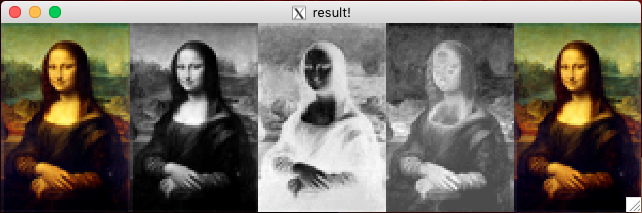
\includegraphics[width=0.6\textwidth]{fig/RGB_to_YCbCr.png}
      \centering
      \caption{A homomorphic transformation of Mona Lisa from RGB to YCbCr preserves visual similarity.
      The Y, Cb, and Cr channels are displayed in the middle}
      \label{rgb_to_ycbcr}
    \end{figure}
    \begin{figure}[h]
      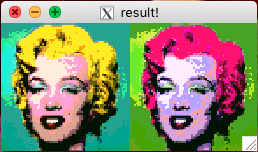
\includegraphics[width=0.45\textwidth]{fig/color_transform.png}
      \centering
      \caption{The input (left) and output (right) of an arbitrary homomorphic color transformation.}
      \label{color}
    \end{figure}
    \begin{figure}[h]
      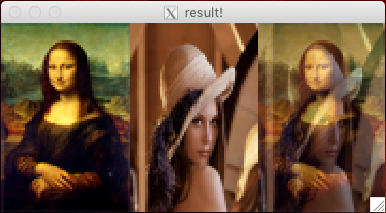
\includegraphics[width=0.6\textwidth]{fig/mean.png}
      \centering
      \caption{A linear mixture of Mona Lisa and Lena, computed homomorphically.}
      \label{mean}
    \end{figure}
    \begin{table}[h]
        \begin{center}
            \begin{tabular}{| c | r | r |}
                \hline
                $\#$ & Time/Batch & Time/Operation
                \\ \hline
                \multicolumn{3}{|c|}{Encryption}
                \\ \hline
                $1$ & \SI{6659.2}{\milli\second} & \SI{1.239}{\milli\second}
                \\ \hline
                $2$ & \SI{6648.9}{\milli\second} & \SI{1.237}{\milli\second}
                \\ \hline
                $3$ & \SI{38263.2}{\milli\second} & \SI{3.559}{\milli\second}
                \\ \hline
                \multicolumn{3}{|c|}{Decryption}
                \\ \hline
                $1$ & \SI{9938.4}{\milli\second} & \SI{1.849}{\milli\second}
                \\ \hline
                $2$ & \SI{9958.3}{\milli\second} & \SI{1.852}{\milli\second}
                \\ \hline
                $3$ & \SI{39974.1}{\milli\second} & \SI{3.718}{\milli\second}
                \\ \hline
                \multicolumn{3}{|c|}{Addition with Constant}
                \\ \hline
                $1$ & \SI{18.4}{\micro\second} & \SI{3.423}{\nano\second}
                \\ \hline
                $2$ & \SI{16.6}{\micro\second} & \SI{3.088}{\nano\second}
                \\ \hline
                $3$ & \SI{27.2}{\micro\second} & \SI{2.530}{\nano\second}
                \\ \hline
                \multicolumn{3}{|c|}{Multiplication with Constant}
                \\ \hline
                $1$ & \SI{1974.2}{\micro\second} & \SI{367.2}{\nano\second}
                \\ \hline
                $2$ & \SI{2186.9}{\micro\second} & \SI{406.8}{\nano\second}
                \\ \hline
                $3$ & \SI{5496.7}{\micro\second} & \SI{511.1}{\nano\second}
                \\ \hline
                \multicolumn{3}{|c|}{Addition of Ciphertexts}
                \\ \hline
                $1$ & \SI{417.6}{\micro\second} & \SI{77.679}{\nano\second}
                \\ \hline
                $2$ & \SI{501.6}{\micro\second} & \SI{93.304}{\nano\second}
                \\ \hline
                $3$ & \SI{6099.4}{\micro\second} & \SI{567.281}{\nano\second}
                \\ \hline
                \multicolumn{3}{|c|}{Multiplication of Ciphertexts}
                \\ \hline.
                $1$ & \SI{462.0}{\milli\second} & \SI{85.932}{\micro\second}
                \\ \hline
                $2$ & \SI{560.7}{\milli\second} & \SI{104.288}{\micro\second}
                \\ \hline
                $3$ & \SI{2306.4}{\milli\second} & \SI{214.511}{\micro\second}
                \\ \hline
                \multicolumn{3}{|c|}{Random Single Variable Function}
                \\ \hline
                $1$ & \SI{20248.2}{\milli\second} & \SI{3.766}{\milli\second}
                \\ \hline
                $2$ & \SI{25029.7}{\milli\second} & \SI{4.656}{\milli\second}
                \\ \hline
                $3$ & \SI{91361.1}{\milli\second} & \SI{8.497}{\milli\second}
                \\ \hline
                \multicolumn{3}{|c|}{Comparison of Ciphertexts}
                \\ \hline
                $2$ & \SI{71071.4}{\milli\second} & \SI{13.220}{\milli\second}
                \\ \hline
                $3$ & \SI{300576}{\milli\second} & \SI{27.955}{\milli\second}
                \\ \hline
                \multicolumn{3}{|c|}{Division of Ciphertexts}
                \\ \hline
                $3$ & \SI{294826}{\milli\second} & \SI{27.688}{\milli\second}
                \\ \hline
            \end{tabular}
        \end{center}
        \label{results}
        \caption{Timing results from the parameters in table~\ref{param}.}
      \end{table}

\end{document}
